
\documentclass{article}

% ---------------------------------------------------------------------------
% ICLR 2027 workshop version: four pages of main text, references and appendix
% unlimited. The conference version is main.tex; every number here is quoted
% from it. Anonymized for double-blind review.
% This file is the source: scripts/build_workshop.py fills the %%BLOCK%% lines
% from main.tex and writes workshop.tex. Edit this file, not workshop.tex.
% Compile:  pdflatex workshop && bibtex workshop && pdflatex workshop x2
% ---------------------------------------------------------------------------

\usepackage{iclr2027_conference,times}
\usepackage{amsmath,amssymb,amsthm}
\usepackage{graphicx}
\usepackage{booktabs}
\usepackage{caption}
\usepackage{xcolor}
\usepackage[colorlinks=true,linkcolor=blue,citecolor=blue,urlcolor=blue]{hyperref}
\usepackage{enumitem}

\graphicspath{{figures/}}

\theoremstyle{plain}
\newtheorem{proposition}{Proposition}
\newtheorem{theorem}{Theorem}
\newtheorem{lemma}{Lemma}
\newtheorem{corollary}{Corollary}
\theoremstyle{remark}
\newtheorem{remark}{Remark}

%%%%% MATH DEFINITIONS, shared by the body and Appendix A %%%%%
% Read by main.tex with %%%%% MATH DEFINITIONS, shared by the body and Appendix A %%%%%
% Read by main.tex with %%%%% MATH DEFINITIONS, shared by the body and Appendix A %%%%%
% Read by main.tex with \input{math_commands}. Proofs use the shorthands at the end,
% so that a display is a line of mathematics and not a line of \frac's.

% --- sets and operators ---------------------------------------------------
\newcommand{\R}{\mathbb{R}}
\newcommand{\E}{\mathbb{E}}
\newcommand{\Var}{\operatorname{Var}}
\newcommand{\Cov}{\operatorname{Cov}}
\newcommand{\tr}{\operatorname{tr}}
\newcommand{\N}{\mathcal{N}}
\newcommand{\D}{\mathcal{D}}
\newcommand{\dist}{\operatorname{dist}}
\newcommand{\supp}{\operatorname{supp}}
\newcommand{\law}{\mathrm{Law}}
\newcommand{\ind}{\mathbf{1}}
\newcommand{\eps}{\varepsilon}

% --- objects of the paper -------------------------------------------------
\newcommand{\Sigmapost}{\Sigma_{\mathrm{post}}}
\newcommand{\Xhat}{\widehat{\Sigma}_X}
\newcommand{\rhohat}{\widehat{\rho}}
\newcommand{\vstar}{v_h^\star}
\newcommand{\vstarz}{v_0^\star}
\newcommand{\Covh}{\operatorname{Cov}_h}

% --- shorthands for the proofs --------------------------------------------
% label weight and kernel weight of atom #1 at bandwidth h
\newcommand{\pih}[1]{p_{#1}^{(h)}}
\newcommand{\wih}[1]{w_{#1}^{(h)}}
% label kernel K_h(y - y^i)
\newcommand{\KK}[1]{K_h(y-y^{#1})}
% per-atom collapsed field (x^i - x)/(1 - t)
\newcommand{\fat}[1]{\frac{x^{#1}-x}{1-t}}
% source density at the point that reaches x from atom #1
\newcommand{\src}[1]{\pi_0\!\Big(\frac{x-tx^{#1}}{1-t}\Big)}

% --- pointer from a statement in the body to its proof --------------------
\newcommand{\proofin}[1]{\hfill\textnormal{\footnotesize[Proof: Appendix~\ref{#1}]}}
. Proofs use the shorthands at the end,
% so that a display is a line of mathematics and not a line of \frac's.

% --- sets and operators ---------------------------------------------------
\newcommand{\R}{\mathbb{R}}
\newcommand{\E}{\mathbb{E}}
\newcommand{\Var}{\operatorname{Var}}
\newcommand{\Cov}{\operatorname{Cov}}
\newcommand{\tr}{\operatorname{tr}}
\newcommand{\N}{\mathcal{N}}
\newcommand{\D}{\mathcal{D}}
\newcommand{\dist}{\operatorname{dist}}
\newcommand{\supp}{\operatorname{supp}}
\newcommand{\law}{\mathrm{Law}}
\newcommand{\ind}{\mathbf{1}}
\newcommand{\eps}{\varepsilon}

% --- objects of the paper -------------------------------------------------
\newcommand{\Sigmapost}{\Sigma_{\mathrm{post}}}
\newcommand{\Xhat}{\widehat{\Sigma}_X}
\newcommand{\rhohat}{\widehat{\rho}}
\newcommand{\vstar}{v_h^\star}
\newcommand{\vstarz}{v_0^\star}
\newcommand{\Covh}{\operatorname{Cov}_h}

% --- shorthands for the proofs --------------------------------------------
% label weight and kernel weight of atom #1 at bandwidth h
\newcommand{\pih}[1]{p_{#1}^{(h)}}
\newcommand{\wih}[1]{w_{#1}^{(h)}}
% label kernel K_h(y - y^i)
\newcommand{\KK}[1]{K_h(y-y^{#1})}
% per-atom collapsed field (x^i - x)/(1 - t)
\newcommand{\fat}[1]{\frac{x^{#1}-x}{1-t}}
% source density at the point that reaches x from atom #1
\newcommand{\src}[1]{\pi_0\!\Big(\frac{x-tx^{#1}}{1-t}\Big)}

% --- pointer from a statement in the body to its proof --------------------
\newcommand{\proofin}[1]{\hfill\textnormal{\footnotesize[Proof: Appendix~\ref{#1}]}}
. Proofs use the shorthands at the end,
% so that a display is a line of mathematics and not a line of \frac's.

% --- sets and operators ---------------------------------------------------
\newcommand{\R}{\mathbb{R}}
\newcommand{\E}{\mathbb{E}}
\newcommand{\Var}{\operatorname{Var}}
\newcommand{\Cov}{\operatorname{Cov}}
\newcommand{\tr}{\operatorname{tr}}
\newcommand{\N}{\mathcal{N}}
\newcommand{\D}{\mathcal{D}}
\newcommand{\dist}{\operatorname{dist}}
\newcommand{\supp}{\operatorname{supp}}
\newcommand{\law}{\mathrm{Law}}
\newcommand{\ind}{\mathbf{1}}
\newcommand{\eps}{\varepsilon}

% --- objects of the paper -------------------------------------------------
\newcommand{\Sigmapost}{\Sigma_{\mathrm{post}}}
\newcommand{\Xhat}{\widehat{\Sigma}_X}
\newcommand{\rhohat}{\widehat{\rho}}
\newcommand{\vstar}{v_h^\star}
\newcommand{\vstarz}{v_0^\star}
\newcommand{\Covh}{\operatorname{Cov}_h}

% --- shorthands for the proofs --------------------------------------------
% label weight and kernel weight of atom #1 at bandwidth h
\newcommand{\pih}[1]{p_{#1}^{(h)}}
\newcommand{\wih}[1]{w_{#1}^{(h)}}
% label kernel K_h(y - y^i)
\newcommand{\KK}[1]{K_h(y-y^{#1})}
% per-atom collapsed field (x^i - x)/(1 - t)
\newcommand{\fat}[1]{\frac{x^{#1}-x}{1-t}}
% source density at the point that reaches x from atom #1
\newcommand{\src}[1]{\pi_0\!\Big(\frac{x-tx^{#1}}{1-t}\Big)}

% --- pointer from a statement in the body to its proof --------------------
\newcommand{\proofin}[1]{\hfill\textnormal{\footnotesize[Proof: Appendix~\ref{#1}]}}

\renewcommand{\proofin}[1]{\hfill\textnormal{\footnotesize[Proof: Appendix~\ref{app:proofs}]}}

\title{Trained Conditional Flows Memorise\\
at an Effective Bandwidth}

\author{Anonymous authors \\ Paper under double-blind review}

\begin{document}
\maketitle

\begin{abstract}
With the training set fixed, the population minimiser of conditional flow matching
sends a condition that identifies one example to that example, and Gaussian noise on
the condition turns its endpoint into a Nadaraya--Watson mixture of the training atoms.
We show that trained networks follow this mixture at one \emph{effective bandwidth}
$h_{\mathrm{eff}}$, fitted to their per-condition variances and recovered independently
from their per-condition means (48/48 synthetic and 31/36 CIFAR-10 checkpoints), which
training shrinks towards the bandwidth $h$ of the label noise. We prove when
$h_{\mathrm{eff}}$ is identified and what calibration it implies: for any prior, label
noise moves the coverage of the reference law by at most a total-variation term of
order $h^2/\sigma^2$, and a vanishing effective sample collapses it to zero. From
$h_{\mathrm{eff}}$ alone, the theorem predicts the held-out coverage of 75 trained
checkpoints with $R^2=0.90$, ranking it better than the training loss or the iteration.
\end{abstract}

% ==========================================================================
\section{Introduction}

Flow matching \citep{lipman2023flow,albergo2023building,liu2023rectified} regresses a
velocity field on a path from noise to data. Used for posterior sampling, conditional
flow matching is calibrated early in training and then becomes nearly deterministic,
returning training examples \citep{physicscfm2026}. That the empirical minimiser
memorises is known for unconditional models
\citep{gao2024flow,bertrand2025closed,kamb2024creativity,buchanan2025edge,li2026memory}.
We ask what the \emph{conditional} minimiser does, what the usual fix, Gaussian noise on
the condition \citep{ho2022cascaded,sadat2024cads}, buys, and how far a trained network
is from either (Figure~\ref{fig:mechanism}). Our contributions:
\begin{itemize}[leftmargin=1.4em,itemsep=1pt,topsep=2pt]
\item \textbf{An exact reference.} A condition that identifies its example is sent to it;
  label noise at bandwidth $h$ gives a Nadaraya--Watson (NW) mixture of the training
  atoms, atomic at every $h$ (Section~\ref{sec:theory}).
\item \textbf{One number per checkpoint.} A trained network follows that mixture at one
  bandwidth $h_{\mathrm{eff}}$, identified by two disjoint statistics; we prove when it
  is identified (Section~\ref{sec:heff}).
\item \textbf{A calibration theorem.} The bandwidth sets the coverage of credible
  regions, for any prior, and predicts the measured coverage of trained models
  (Section~\ref{sec:calib}).
\end{itemize}

\begin{figure}[t]
\centering
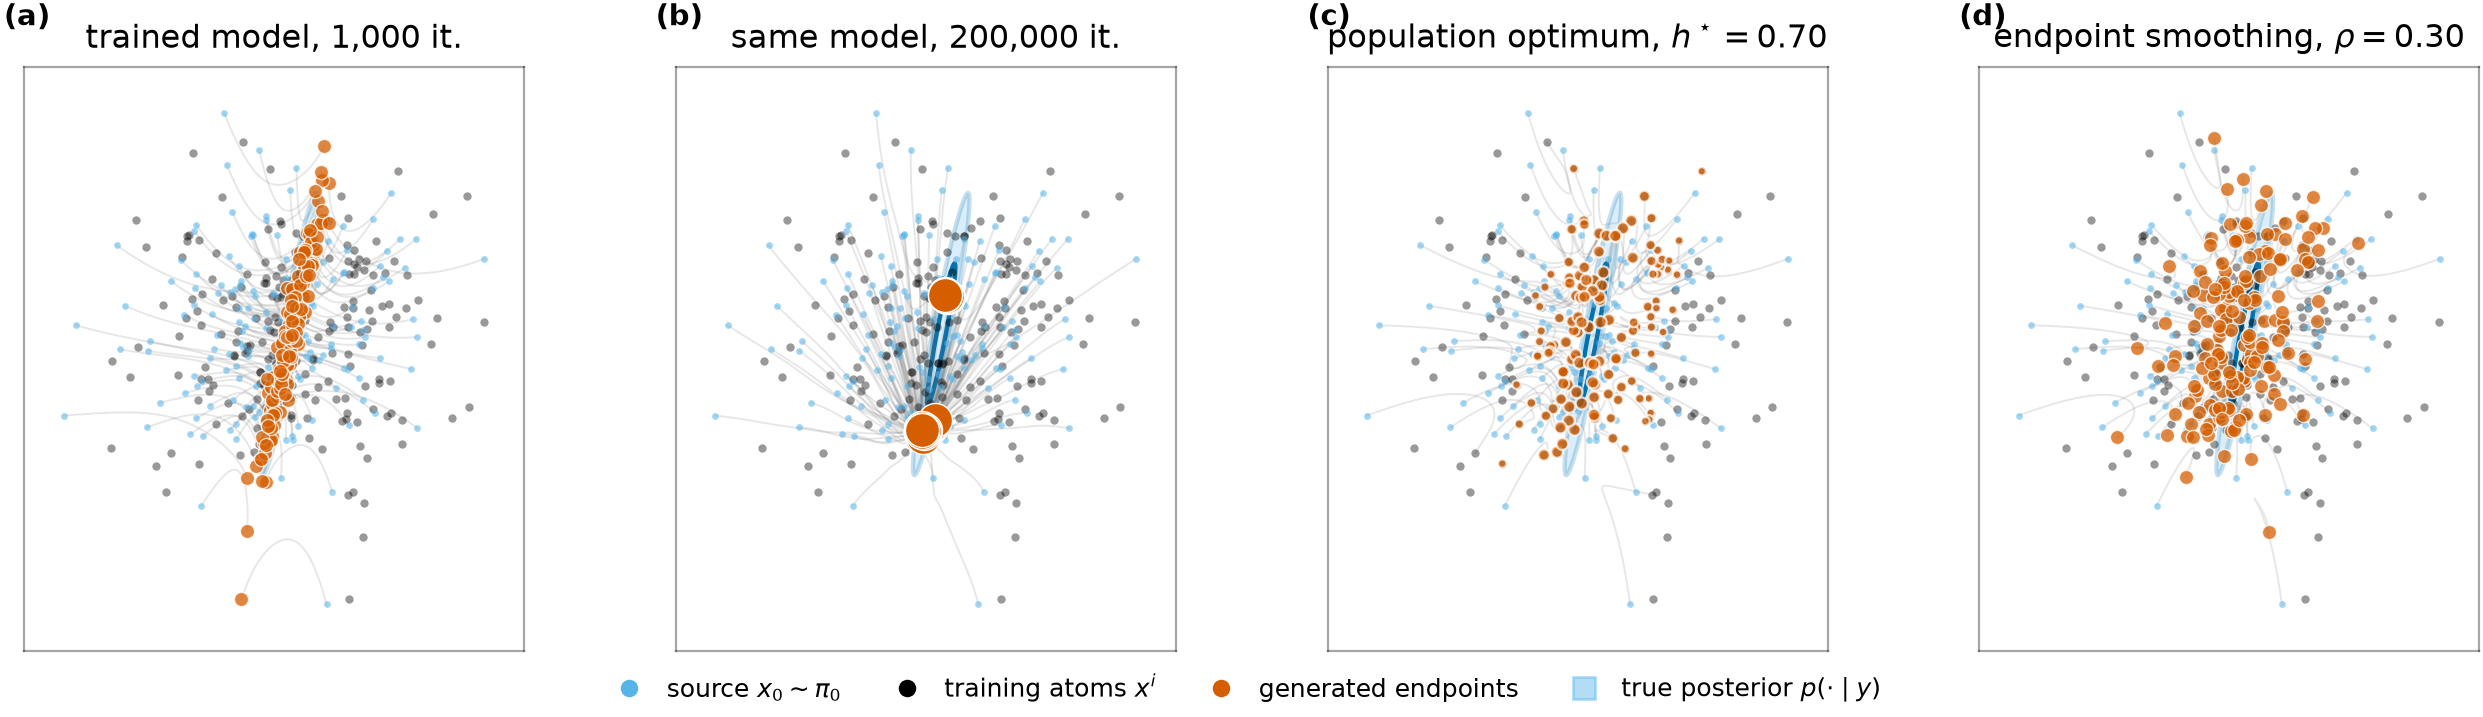
\includegraphics[width=\textwidth]{fig_flow_portrait.png}
\caption{One condition of the synthetic instance ($d{=}2$, $N{=}200$), $160$ source
draws. (a,~b) A trained network at $10^3$ and $2\times10^5$ iterations: first a
posterior sampler, then $96\%$ of paths end on the labelled atom. (c) The population
optimum at the bandwidth whose $\tr\Covh$ equals $\tr\Sigmapost$; marker area is
$p_i^{(h)}$. The variance is right and the law is still atomic. (d) Endpoint noise
leaves the atoms.}
\label{fig:mechanism}
\end{figure}

% ==========================================================================
\section{The exact reference}
\label{sec:theory}

Fix $\D=\{(x^i,y^i)\}_{i=1}^N$, $x^i\in\R^d$, with distinct labels $y^i\in\R^k$, as in
inverse problems and inpainting. Draw $I\sim\mathrm{Unif}\{1,\dots,N\}$,
$X_0\sim\pi_0=\N(0,I_d)$, $t\sim\mathrm{Unif}(0,1)$, $\eps\sim\N(0,I_k)$; set
$X_t=(1-t)X_0+tx^I$, $U=x^I-X_0$, $\widetilde Y=y^I+h\eps$, and minimise
$\E|U-v(X_t,t,\widetilde Y)|^2$; the minimiser is $\vstar=\E[U\mid X_t,t,\widetilde Y]$.
Write $K_h(u)\propto e^{-|u|^2/2h^2}$ and $p_i^{(h)}(y)=K_h(y-y^i)/\sum_jK_h(y-y^j)$.

\begin{theorem}[Endpoint law]
\label{thm:endpoint}
At $h=0$, $v_0^\star(x,t,y^i)=(x^i-x)/(1-t)$, the loss is zero and every source point
reaches $x^i$. For $h>0$ the flow of $\vstar$ from $\pi_0$ ends at
$p_1(\cdot\mid y)=\sum_ip_i^{(h)}(y)\,\delta_{x^i}$, with moments
$\bar x_h(y)=\sum_ip_i^{(h)}x^i$ and $\Covh(y)=\sum_ip_i^{(h)}(x^i-\bar x_h)(x^i-\bar
x_h)^\top$. It is supported on the atoms at every $h$, so if the posterior gives the
atoms no mass, $W_2^2(p_1,p(\cdot\mid y))\ge\int\dist(x,\{x^i\})^2p(x\mid y)\,dx>0$,
independently of $h$. \proofin{}
\end{theorem}

So label noise matches the posterior's variance at best, never its law. Noise on the
interpolant changes nothing and only noise on the endpoint leaves the atoms
(Appendix~\ref{app:interventions}).

% ==========================================================================
\section{Trained models sit at an effective bandwidth}
\label{sec:heff}

A trained model need not sit at its own training bandwidth. With $T_c$ and $m_c$ its
generated trace and mean at condition $y_c$,
\begin{equation}
h_{\mathrm{eff}}=\arg\min_{h'}\sum_c\big(\log T_c-\log\tr\mathrm{Cov}_{h'}(y_c)\big)^2,
\qquad
h_{\mathrm{mean}}=\arg\min_{h'}\sum_c\big\|m_c-\bar x_{h'}(y_c)\big\|.
\label{eq:heff}
\end{equation}
The two use disjoint statistics, so $h_{\mathrm{mean}}\approx h_{\mathrm{eff}}$ checks
that the model is an NW mixture at all.

\begin{proposition}[Identifiability]
\label{prop:heffid}
With $D_i=|y-y^i|^2$ and $\Cov_p$ the covariance over $i$ under $p^{(h)}(y)$,
$\partial_h\bar x_h=h^{-3}\Cov_p(x^i,D_i)$ and
$\partial_h\tr\Covh=h^{-3}\Cov_p(|x^i-\bar x_h|^2,D_i)$, so the latter is $O(h^{-3})$ as
$h\to\infty$. Let $F(h)=(\log\tr\mathrm{Cov}_h(y_c))_c$, the measured log traces be
$F(h^\star)+e$, and $\hat h$ minimise $|\log T-F(h)|$ over a set $\mathcal H$. Then
$\hat h\in\{h\in\mathcal H:|F(h)-F(h^\star)|\le2|e|\}$; if this set lies in an interval
$\mathcal I\ni h^\star$ on which $u\cdot F'\ge\kappa>0$ for a unit vector $u$, then
$|\hat h-h^\star|\le2|e|/\kappa$. \proofin{}
\end{proposition}

\begin{figure}[t]
\centering
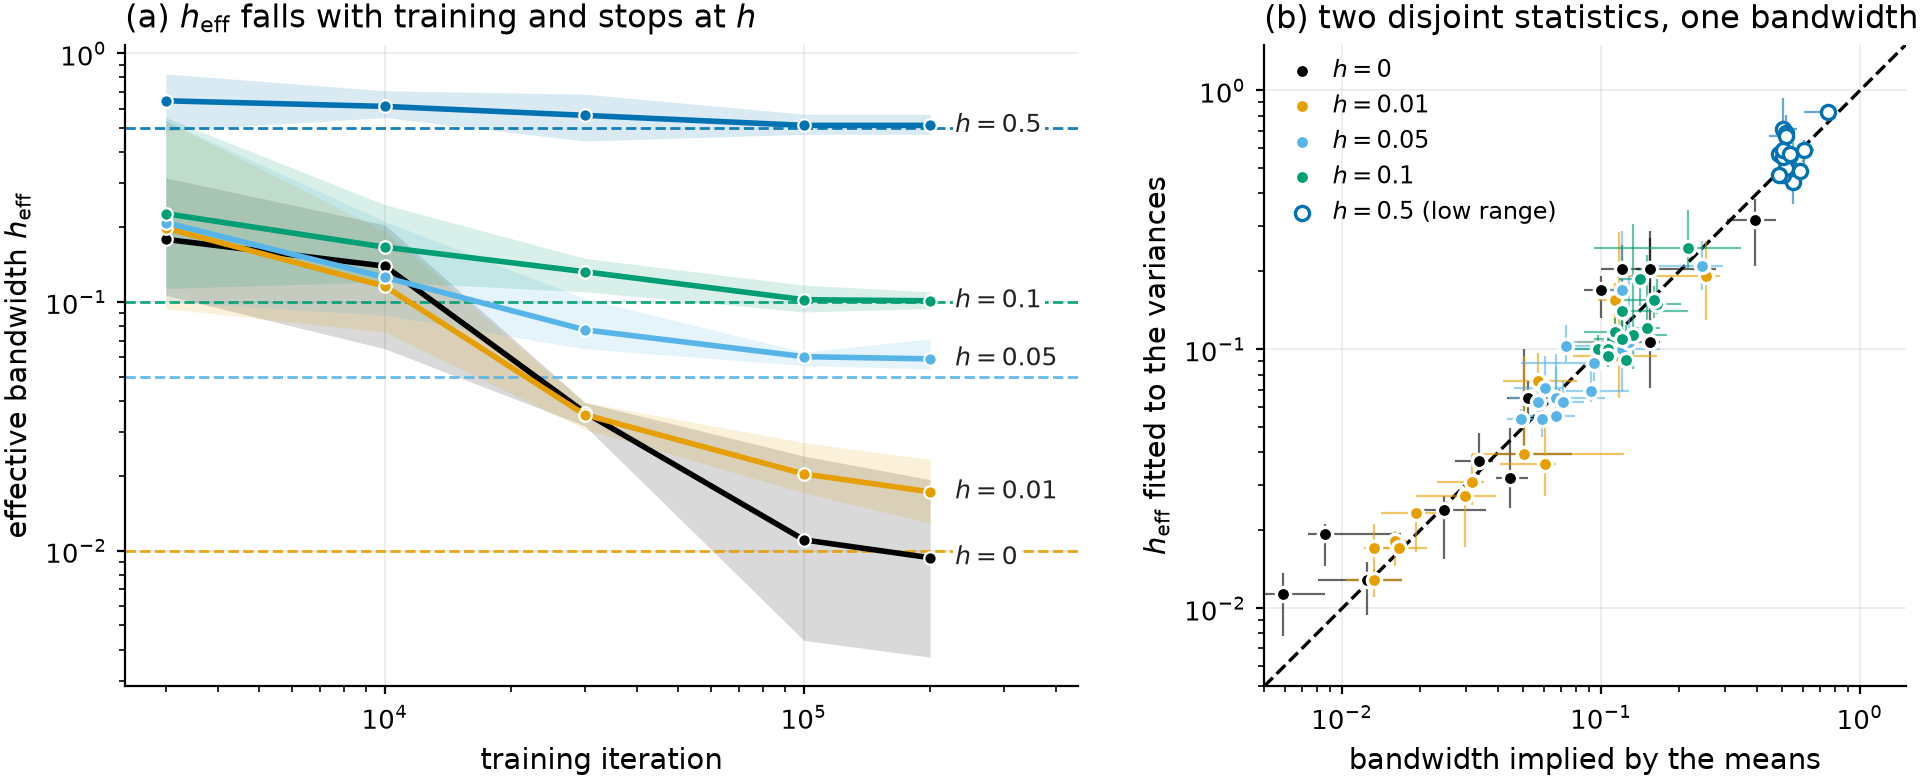
\includegraphics[width=\textwidth]{fig_heff_synthetic.png}
\caption{Linear-Gaussian problem, three seeds per bandwidth. (a) $h_{\mathrm{eff}}$
falls with training and stops just above the training bandwidth $h$ (dashed); line:
geometric mean over seeds, band: range. Checkpoints before 3000 iterations, where no
bandwidth fits, are omitted. (b) The bandwidth fitted to the variances against the one
implied by the means, with 95\% bootstrap intervals: two disjoint statistics give one
bandwidth. Open markers ($h=0.5$): the reference barely varies and
$h_{\mathrm{eff}}$ is poorly identified.}
\label{fig:heffsyn}
\end{figure}

\paragraph{Results.} On a linear-Gaussian problem ($d{=}2$, $N{=}200$; 15 MLP runs,
$h\in\{0,0.01,0.05,0.1,0.5\}$) the two bandwidths agree within 95\% intervals at all
48 checkpoints where the reference varies; $h_{\mathrm{eff}}$ falls between $10^4$ and
$10^5$ iterations and settles at $1.08h$. At $h{=}0.5$ it is poorly identified, as the
proposition predicts ($\kappa$ is $1.4$ there against $5$--$33$ for $h\le0.1$). With a
$35.75$M-parameter DDPM U-Net on CIFAR-10 inpainting ($N{=}2000$, six runs,
$h\in\{4,5\}$) they agree at 31/36 checkpoints, and $h_{\mathrm{eff}}$ falls to
$1.13$--$1.34h$ by 60k iterations (Figure~\ref{fig:heffsyn}; CIFAR-10 in
Figure~\ref{fig:heffcifar}, appendix).

% ==========================================================================
\section{The bandwidth sets calibration}
\label{sec:calib}

\begin{theorem}[Calibration of the reference law]
\label{thm:calib}
Let $X\sim\pi$, $Y=g(X)+\eta$, $\eta\sim\N(0,\sigma^2I_k)$, with $\pi$, $g$ arbitrary,
and $\pi_h(\cdot\mid y)$ the law of $X$ given $Y+h\eps=y$.
(a) For an i.i.d.\ training set, $p_1(\cdot\mid y)\Rightarrow\pi_h(\cdot\mid y)$ as
$N\to\infty$. (b) Level-$\alpha$ regions of $\pi_h$ cover $X$ at the clean label $Y$
with probability within $\tau_h=\mathrm{TV}(\N(0,\sigma^2I),\N(0,(\sigma^2{+}h^2)I))
\le\sqrt{k/8}\,h^2/\sigma^2$ of $\alpha$; (c) if $\pi$ is Gaussian and $g$ linear, at
least $\alpha$. (d) A region built from $n_{\mathrm{eff}}=1/\sum_iw_i^2$ weighted atoms
has expected covariance $(1-1/n_{\mathrm{eff}})S$; at $n_{\mathrm{eff}}=1$ it covers
with probability $0$. \proofin{}
\end{theorem}

\begin{figure}[t]
\centering
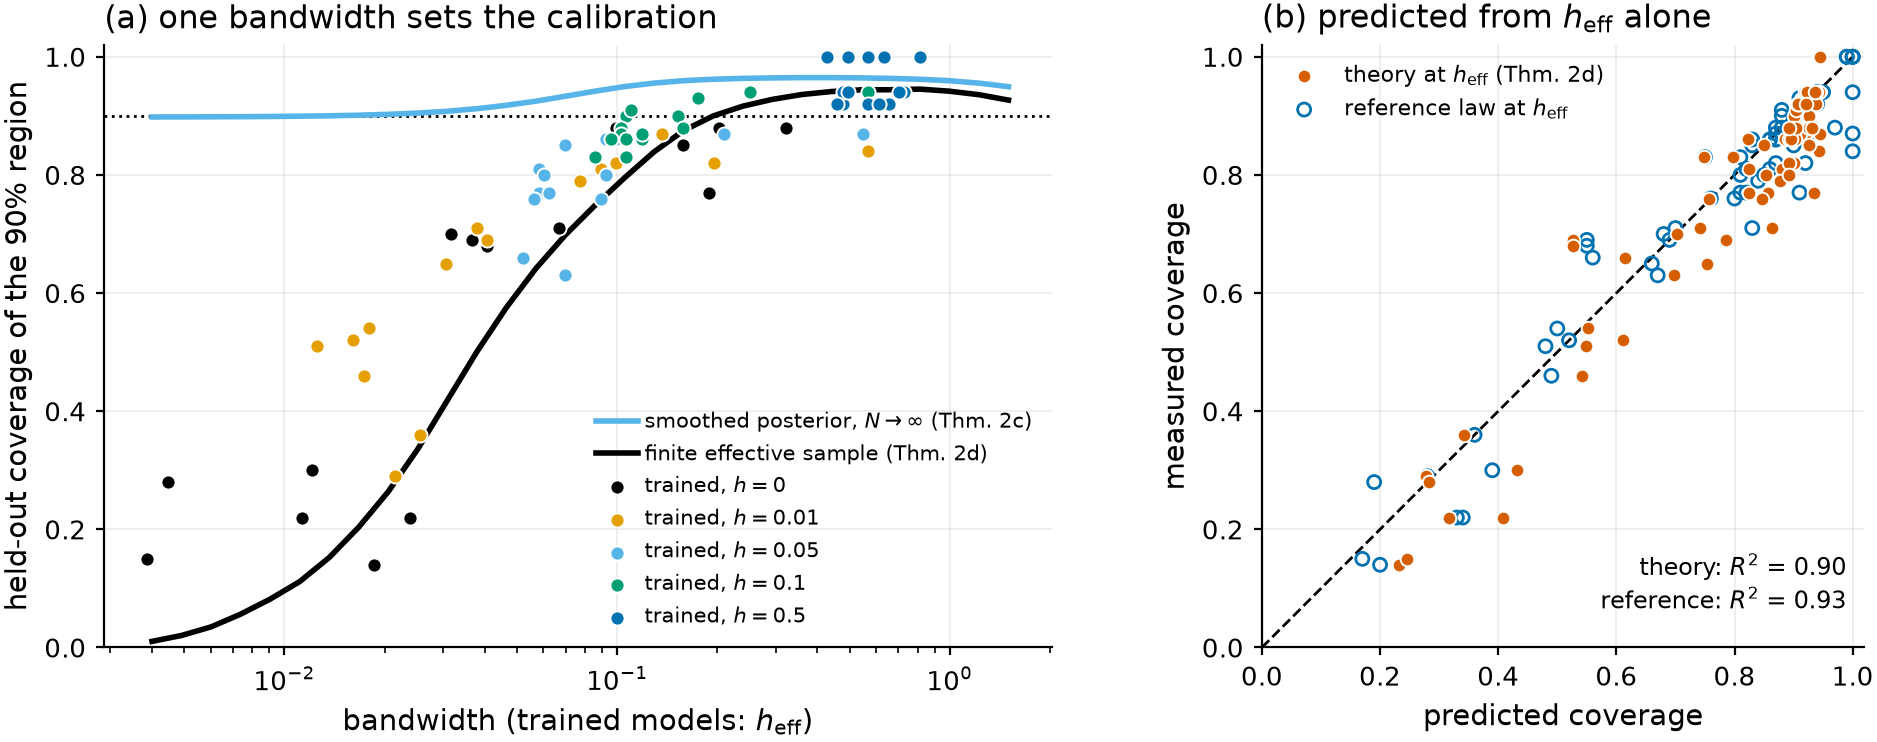
\includegraphics[width=0.92\textwidth]{fig_t3_coverage.png}
\vspace{-3pt}
\caption{Linear-Gaussian problem. (a) Coverage of the nominal 90\% region against
bandwidth: infinite-data limit (Theorem~\ref{thm:calib}c), over-covering for $h>0$;
finite effective sample (d), collapsing at small bandwidth; dots: 75 trained
checkpoints at their $h_{\mathrm{eff}}$. (b) Coverage predicted from $h_{\mathrm{eff}}$
alone against the measured coverage.}
\label{fig:t3}
\end{figure}

Parts (b, c) give the over-coverage edge of a calibration window, (d) the collapse edge.
Modelling the atoms near a held-out $y^\star$ as draws of $\pi_h$ with the actual
weights, (d) predicts the held-out 90\% coverage of all 75 synthetic checkpoints from
their $h_{\mathrm{eff}}$ alone with $R^2=0.90$ (Figure~\ref{fig:t3}). As a ranking,
$h_{\mathrm{eff}}$ (Spearman $0.92$) beats the training loss ($0.85$) and the iteration
($-0.42$), keeps $0.90$ with the iteration partialled out, and repeats on an eight-mode
mixture posterior ($0.91$; Table~\ref{tab:baselines}). On the mixture the
bound (b) holds and is nearly tight at $h=\sigma/2$.

\begin{table}[t]
\centering\small
\setlength{\tabcolsep}{4pt}
\begin{tabular}{lcccccccc}
\toprule
& \multicolumn{4}{c}{linear-Gaussian, $d{=}2$ (75 checkpoints)} &
\multicolumn{4}{c}{Gaussian mixture, $d{=}8$ (50 checkpoints)}\\
\cmidrule(lr){2-5}\cmidrule(l){6-9}
predictor & pooled & $\mid$ iter & $\mid$ iter, $h$ & fixed iter &
pooled & $\mid$ iter & $\mid$ iter, $h$ & fixed iter\\
\midrule
$h_{\mathrm{eff}}$ & \textbf{0.92} & \textbf{0.90} & \textbf{0.69} & \textbf{0.82} &
\textbf{0.91} & \textbf{0.91} & 0.61 & \textbf{0.90}\\
training loss & 0.85 & 0.82 & 0.42 & 0.75 & 0.88 & 0.81 & \textbf{0.62} & 0.81\\
raw trace & 0.76 & 0.73 & 0.32 & 0.70 & 0.69 & 0.70 & 0.41 & 0.71\\
iteration & $-0.42$ & --- & --- & --- & $-0.66$ & --- & --- & ---\\
$\beta$ & 0.34 & 0.54 & $-0.19$ & 0.61 & 0.29 & 0.61 & $-0.45$ & 0.66\\
\bottomrule
\end{tabular}
\caption{Spearman correlation of each statistic, computed from the training set and
the model alone, with the held-out 90\% coverage: pooled; partialling out
$\log$(iteration); partialling out $\log$(iteration) and the training bandwidth $h$;
and averaged across runs at a fixed iteration. $h_{\mathrm{eff}}$ is not a proxy for
training time.}
\label{tab:baselines}
\end{table}

% ==========================================================================
\section{Limitations and conclusion}

Which bandwidth training reaches is measured, not proved: a kernel model of spectral bias
reproduces the fall of $h_{\mathrm{eff}}$ to $h$, and limited label resolution provably
reweights the atoms without moving them (Appendix~\ref{app:specbias}), but neither
explains why networks stop just above $h$. Calibration is shown where the posterior is
known ($d\le8$); at image scale $h_{\mathrm{eff}}$ fits the variances no better than a
power law. Within that scope, the memorisation and calibration of a conditional sampler
are set by one number read off a checkpoint.

\subsection*{Reproducibility and AI use statements}
All numbers are produced by code in the supplementary material (anonymized), and full
proofs are in Appendix~\ref{app:proofs}. A generative-AI assistant was used to draft and
edit text, to expand proofs into their full form, to write the training and analysis
code, and to run and analyse experiments. Every reported number is produced by the
released code from actual runs; the authors checked all proofs and results and take full
responsibility for the content.

\bibliographystyle{plainnat}
\bibliography{refs}

% ==========================================================================
\appendix
\section{Proofs}
\label{app:proofs}

Throughout, conditionally on $I=i$ and for $t<1$ the map $X_0\mapsto X_t$ is an affine
bijection, so $p(x\mid I=i,t)=(1-t)^{-d}\pi_0\big(\tfrac{x-tx^i}{1-t}\big)>0$, and the
factor $(1-t)^{-d}$ cancels in every posterior over $I$. Every field below has the form
$\sum_iw_i(x,t)(x^i-x)/(1-t)$ with smooth weights in $[0,1]$ summing to one; it is
therefore locally Lipschitz on $\R^d\times[0,1)$ with $|v|\le(|x|+\max_i|x^i|)/(1-t)$,
so by Gr\"onwall each trajectory exists on $[0,1)$ and the push-forward of $\pi_0$ is the
unique solution of the continuity equation there \citep[Ch.~8]{ambrosio2008gradient}.

\paragraph{Projection.} For $m=\E[U\mid X_t,t,\widetilde Y]$,
$L_h(v)=\E|U-m|^2+\E|v-m|^2$, since the cross term vanishes by the tower property; so
$\vstar=m$ a.e.\ and $\inf_vL_h=\E\Var(U\mid X_t,t,\widetilde Y)$.

\begin{proof}[Proof of Theorem~\ref{thm:endpoint}, $h=0$]
Distinct labels give $I=i$ from $Y=y^i$, and then $X_0=(X_t-tx^i)/(1-t)$, so
$U=x^i-X_0=(x^i-X_t)/(1-t)$ is a function of the conditioning variables. Hence
$v_0^\star=(x^i-x)/(1-t)$ and $L_0(v_0^\star)=0$. Along
$\dot x_t=(x^i-x_t)/(1-t)$, $\frac{d}{dt}\frac{x_t-x^i}{1-t}=0$, so
$x_t=(1-t)x_0+tx^i\to x^i$ for every $x_0$, and $p_1=\delta_{x^i}$.
\end{proof}

\begin{proof}[Proof of Theorem~\ref{thm:endpoint}, $h>0$]
Given $I=i$, $X_t$ and $\widetilde Y$ are independent, so by Bayes
$\Pr(I=i\mid X_t=x,t,\widetilde Y=y)\propto\pi_0\big(\tfrac{x-tx^i}{1-t}\big)K_h(y-y^i)=:w_i$,
and $U=(x^i-x)/(1-t)$ given $I=i$, $X_t=x$; this gives the field. Now fix $y$ and
consider the coupling $J\sim p^{(h)}(y)$, $X_0\sim\pi_0$ independent, $X_1=x^J$,
$X_t=(1-t)X_0+tX_1$. Its index posterior is
$\propto p_i^{(h)}(y)\pi_0\big(\tfrac{x-tx^i}{1-t}\big)\propto w_i$, so
$\E[X_1-X_0\mid X_t=x,t]=\vstar(x,t,y)$. For $\varphi\in C_c^\infty$,
$\frac{d}{dt}\E\varphi(X_t)=\E\langle\nabla\varphi(X_t),X_1-X_0\rangle
=\E\langle\nabla\varphi(X_t),\vstar(X_t,t,y)\rangle$, so $\law(X_t)$ solves the
continuity equation of the flow from $\pi_0$ and, by uniqueness, equals the flow's
marginal. Since $X_t\to x^J$ almost surely, $p_1=\law(x^J)=\sum_ip_i^{(h)}(y)\delta_{x^i}$.
The moments follow. As $h\to0$ with a unique nearest label $i^\star$,
$K_h(y-y^i)/K_h(y-y^{i^\star})\to0$ for $i\ne i^\star$; as $h\to\infty$,
$p_i^{(h)}\to1/N$.
\end{proof}

\begin{proof}[Proof of the floor in Theorem~\ref{thm:endpoint}]
The support statement is the endpoint law. For any coupling $(X,X')$ of
$p_1(\cdot\mid y)$ and $p(\cdot\mid y)$, $X\in\{x^i\}$ almost surely, so
$\E|X-X'|^2\ge\E\dist(X',\{x^i\})^2=:F(y)$; take the infimum over couplings. $F$
involves only the atoms and the posterior, and is positive because the atoms are
$p(\cdot\mid y)$-null.
\end{proof}

\begin{proof}[Proof of Proposition~\ref{prop:interp}]
Given $I=i$, $r:=x-tx^i=(1-t)X_0+\gamma Z\sim\N(0,s_t^2I_d)$, so
$\E[X_0\mid r]=\frac{1-t}{s_t^2}r$ and $\E[Z\mid r]=\frac{\gamma}{s_t^2}r$. Hence
$v^\star_\sigma(x,t,y^i)=x^i+c(t)(x-tx^i)$ with
$c=\frac{-(1-t)+\gamma\dot\gamma}{s_t^2}=\frac12\frac{d}{dt}\log s_t^2$. Then
$u_t=x_t-tx^i$ solves $\dot u=c(t)u$, so $u_t=s_tx_0$ (as $s_0=1$). Finally
$s_t^2=(1-t)[(1-t)+\sigma^2t]$, so $s_1=0$ and $x_t\to x^i$.
\end{proof}

\begin{proof}[Proof of Proposition~\ref{prop:endpointnoise}]
Given $I=i$, $r:=x-tx^i=(1-t)X_0+t\rho\xi\sim\N(0,s_t^2I_d)$ with
$s_t^2=(1-t)^2+t^2\rho^2$, so the index posterior is
$\propto\varphi_{s_t}(x-tx^i)K_h(y-y^i)$ and, by Gaussian conditioning,
$\E[U\mid X_t=x,t,I=i]=x^i+\frac{t\rho^2-(1-t)}{s_t^2}(x-tx^i)$. This field is smooth
on $\R^d\times[0,1]$ since $s_1=\rho>0$. The coupling $J\sim p^{(h)}(y)$,
$X_1=x^J+\rho\xi$ has the same index posterior and conditional velocity, so, as in the
proof of Theorem~\ref{thm:endpoint}, $p_1=\law(x^J+\rho\xi)=\sum_ip_i^{(h)}\N(x^i,\rho^2I_d)$,
with mean $\bar x_h$ and covariance $\Covh+\rho^2I_d$.
\end{proof}

%%BLOCK:proof_heffid%%

%%BLOCK:proof_calib%%

The numerical checks of every part are in \texttt{scripts/theory\_t1\_check.py},
\texttt{theory\_t3\_coverage.py} and \texttt{theory\_t3\_general.py}.

\section{Where noise enters}
\label{app:interventions}

\begin{table}[t]
\centering\small
\begin{tabular}{@{}llll@{}}
\toprule
noise on & population endpoint law & effect & result\\
\midrule
interpolant, $\gamma(t)=\sigma\sqrt{t(1-t)}$ & $\delta_{x^i}$ for every $\sigma$ & none &
Prop.~\ref{prop:interp}\\
label, bandwidth $h$ & $\sum_ip_i^{(h)}\delta_{x^i}$ & reweights atoms &
Thm.~\ref{thm:endpoint}\\
endpoint, $X_1=x^I+\rho\xi$ & $\sum_ip_i^{(h)}\N(x^i,\rho^2I_d)$ & moves support,
$+\rho^2I_d$ & Prop.~\ref{prop:endpointnoise}\\
\bottomrule
\end{tabular}
\caption{Where noise enters, and what it does to the population endpoint law. Only
endpoint noise yields an absolutely continuous law, to which the floor of Theorem~\ref{thm:endpoint} does not
apply; it pays for continuity in variance.}
\label{tab:interventions}
\end{table}

\begin{proposition}[Interpolant noise]
\label{prop:interp}
Let $h=0$, $X_t=(1-t)X_0+tx^I+\gamma(t)Z$ with $Z\sim\N(0,I_d)$ and target
$\dot X_t=x^I-X_0+\dot\gamma(t)Z$. With $s_t^2=(1-t)^2+\gamma(t)^2$ the optimal flow is
$x_t=tx^i+s_tx_0$; since $s_1=0$, $p_1(\cdot\mid y^i)=\delta_{x^i}$ for every
$\sigma\ge0$.
\end{proposition}

\begin{proposition}[Endpoint noise]
\label{prop:endpointnoise}
With $X_1=x^I+\rho\xi$, $\xi\sim\N(0,I_d)$ redrawn at every step and $h>0$, the endpoint
law is $\sum_ip_i^{(h)}(y)\N(x^i,\rho^2I_d)$, with mean $\bar x_h(y)$ and covariance
$\Covh(y)+\rho^2I_d$.
\end{proposition}

\section{Additional results}
\label{app:results}

\begin{table}[t]
\centering\small
\begin{tabular}{lcccccc}
\toprule
$h_{\mathrm{eff}}$ & $<0.02$ & $[0.02,0.05)$ & $[0.05,0.1)$ & $[0.1,0.2)$ & $[0.2,0.4)$ &
$\ge0.4$\\
\midrule
checkpoints & 9 & 9 & 14 & 20 & 5 & 18\\
90\% coverage (nominal $0.90$) & 0.34 & 0.54 & 0.79 & \textbf{0.86} & \textbf{0.88} & 0.94\\
calibration error & 0.94 & 0.63 & 0.22 & \textbf{0.10} & \textbf{0.10} & 0.16\\
\bottomrule
\end{tabular}
\caption{Held-out calibration against $h_{\mathrm{eff}}$ on the linear-Gaussian problem
(15 runs, 75 checkpoints, 100 held-out pairs each). Calibration error is
$|c_{50}-0.5|+|c_{90}-0.9|$ for the coverages $c_{50},c_{90}$ of the 50\% and 90\%
regions. Too small an $h_{\mathrm{eff}}$ under-covers (collapse); too large
over-covers.}
\label{tab:calib}
\end{table}

\begin{figure}[t]
\centering
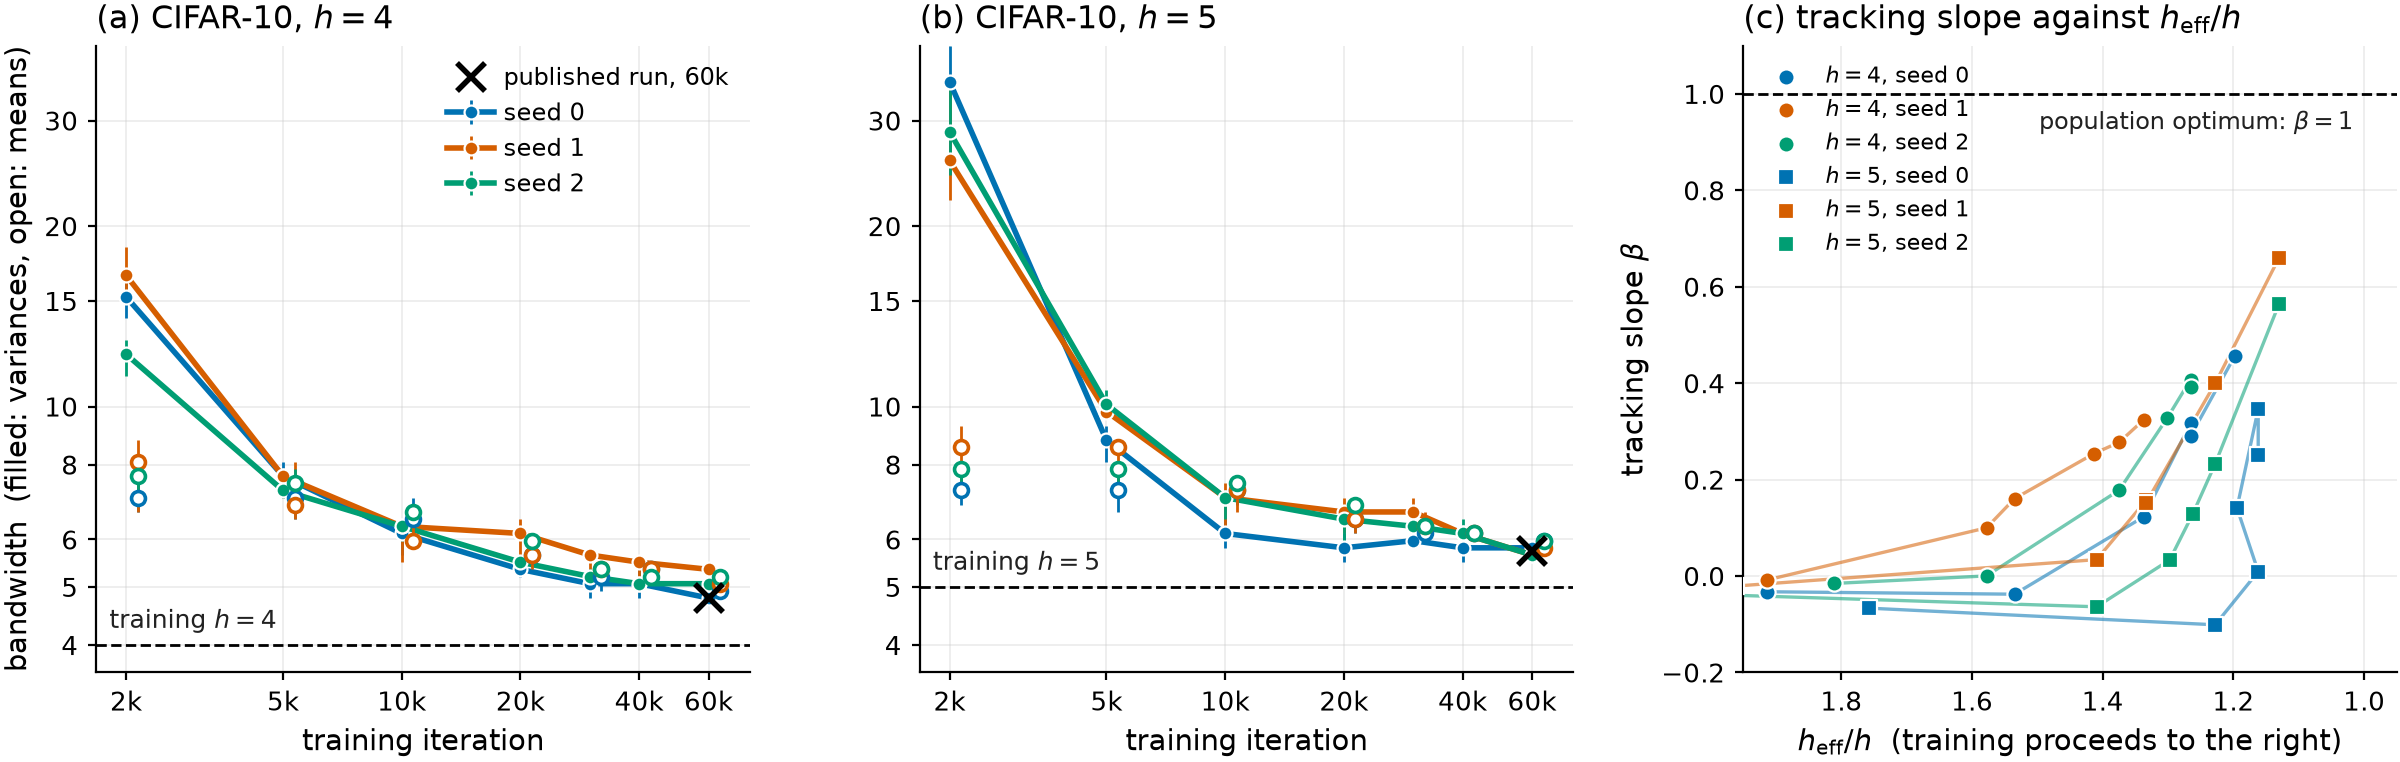
\includegraphics[width=\textwidth]{fig_heff_cifar.png}
\caption{CIFAR-10, DDPM U-Net, three instances per bandwidth. (a, b) $h_{\mathrm{eff}}$
from the variances (filled) and the bandwidth implied by the means (open), with 95\%
intervals, against training iteration; dashed: training $h$; cross: the published run
at 60k. From 5k on the two agree and fall towards $h$ without reaching it. (c) The
tracking slope $\beta$ against $h_{\mathrm{eff}}/h$; training proceeds to the right.}
\label{fig:heffcifar}
\end{figure}

\section{Where the bandwidth comes from}
\label{app:specbias}

%%BLOCK:specbias%%

\end{document}
